\documentclass[10pt,aspectratio=169]{beamer}
\usepackage{booktabs}
\usepackage{graphicx}
\usepackage{tikz}

\usetheme{default}
\usecolortheme{dove}
\beamertemplatenavigationsymbolsempty
\setbeamertemplate{footline}[frame number]

\title{Stopping Target Geometry Optimization for Run~1A CE}
\subtitle{Autoresearch loop: LLM-greedy \texorpdfstring{$\to$}{->} Bayesian Optimization}
\author{O. Oksuzian}
\institute{Mu2e}
\date{\today}

\begin{document}

% ----------------------------------------------------------------
\begin{frame}\titlepage\end{frame}

% ----------------------------------------------------------------
\begin{frame}{Goal and metric}
Maximize \textbf{Run~1A Coherent Electron $S/\sqrt{B}$} by varying the muon
stopping-target geometry.

\medskip
\begin{itemize}
\item Single scalar metric:
      $S/\sqrt{B}$ from \texttt{rough\_run1a\_sensitivity.C}
\item Per-config window scan picks optimal $[x_1, x_2]$ in $p$-space
\item Cosmic background is \emph{hard-coded} in the analysis macro
      ($\sim 1.8 \times 10^{-3}$ ev/s/MeV/c)
\item DIO $\ll$ cosmic above 100 MeV/c $\Rightarrow$ optimum is essentially
      \emph{signal acceptance / window-width tradeoff}
\end{itemize}
\end{frame}

% ----------------------------------------------------------------
\begin{frame}{Running-period assumption (in \texttt{rough\_run1a\_sensitivity.C})}
All $S/\sqrt{B}$ values are computed at a \emph{fixed} hypothetical exposure:

\medskip
\begin{tabular}{lll}
\toprule
Quantity & Value & Note \\
\midrule
$N(\mathrm{POT})$       & $10^{18}$              & assumed exposure \\
Beam mode               & 1BB                   & $1.6\times 10^{7}$ POT/event \\
Simulated events        & $6.25\times 10^{10}$  & derived \\
On-spill seconds        & $\sim 1.06\times 10^{5}$ s & $\sim 29.4$ h beam-on \\
$R_{\mu e}$ assumption  & $10^{-9}$             & signal hypothesis \\
$\mathrm{BR}(\mu\text{-capture, Al})$ & $0.609$ & for signal branching \\
Cosmic rate (hard-coded)& $\sim 1.8\times 10^{-3}$/s/MeV/c & not from sim \\
\bottomrule
\end{tabular}

\medskip
\textbf{Context:} $10^{18}$ POT is $\sim 10\times$ actual Run~1A exposure.
The number is a normalization that scales signal/DIO/cosmic the same way; only
ratios across configs matter for the optimization.

\smallskip
To project to real Run~1A: multiply $S/\sqrt{B}$ by $\sqrt{N_{\mathrm{actual}}/10^{18}} \approx 0.32$.
$\Rightarrow$ baseline 3.31 $\to$ $\sim 1.0$; optimum 3.81 $\to$ $\sim 1.2$ at real Run~1A.
\end{frame}

% ----------------------------------------------------------------
\begin{frame}{Per-evaluation pipeline ($\sim$20 min on 30 cores)}
\begin{enumerate}
\item Fork from \texttt{config\_v00} (37-foil baseline) via \texttt{new\_config.sh}
\item Override target geometry in \texttt{config\_<X>/run1a\_beam/geom.txt}
\item Stage \texttt{run1a\_mubeam}: 30 jobs $\times$ 5\,k events
      (G4 muon beam $\to$ TargetStops)
\item Stage \texttt{run1a\_mustops}: 30 jobs $\times$ 10\,k events,
      modes \{ce, flat\_gamma, flat\_electron\}
\item Read $S/\sqrt{B}$ from \texttt{rough\_run1a\_sensitivity.log}
\end{enumerate}

\medskip
Workdir setup: prepend our tree to \texttt{FHICL\_FILE\_PATH} and
\texttt{MU2E\_SEARCH\_PATH}; reuse \texttt{mmackenz/run1b/} for the \texttt{czMin}-patched
Offline source and pre-built \texttt{EdepAna\_module.so}.
\end{frame}

% ----------------------------------------------------------------
\begin{frame}{Autoresearch pipeline: outer loop + per-evaluation data flow}
\centering
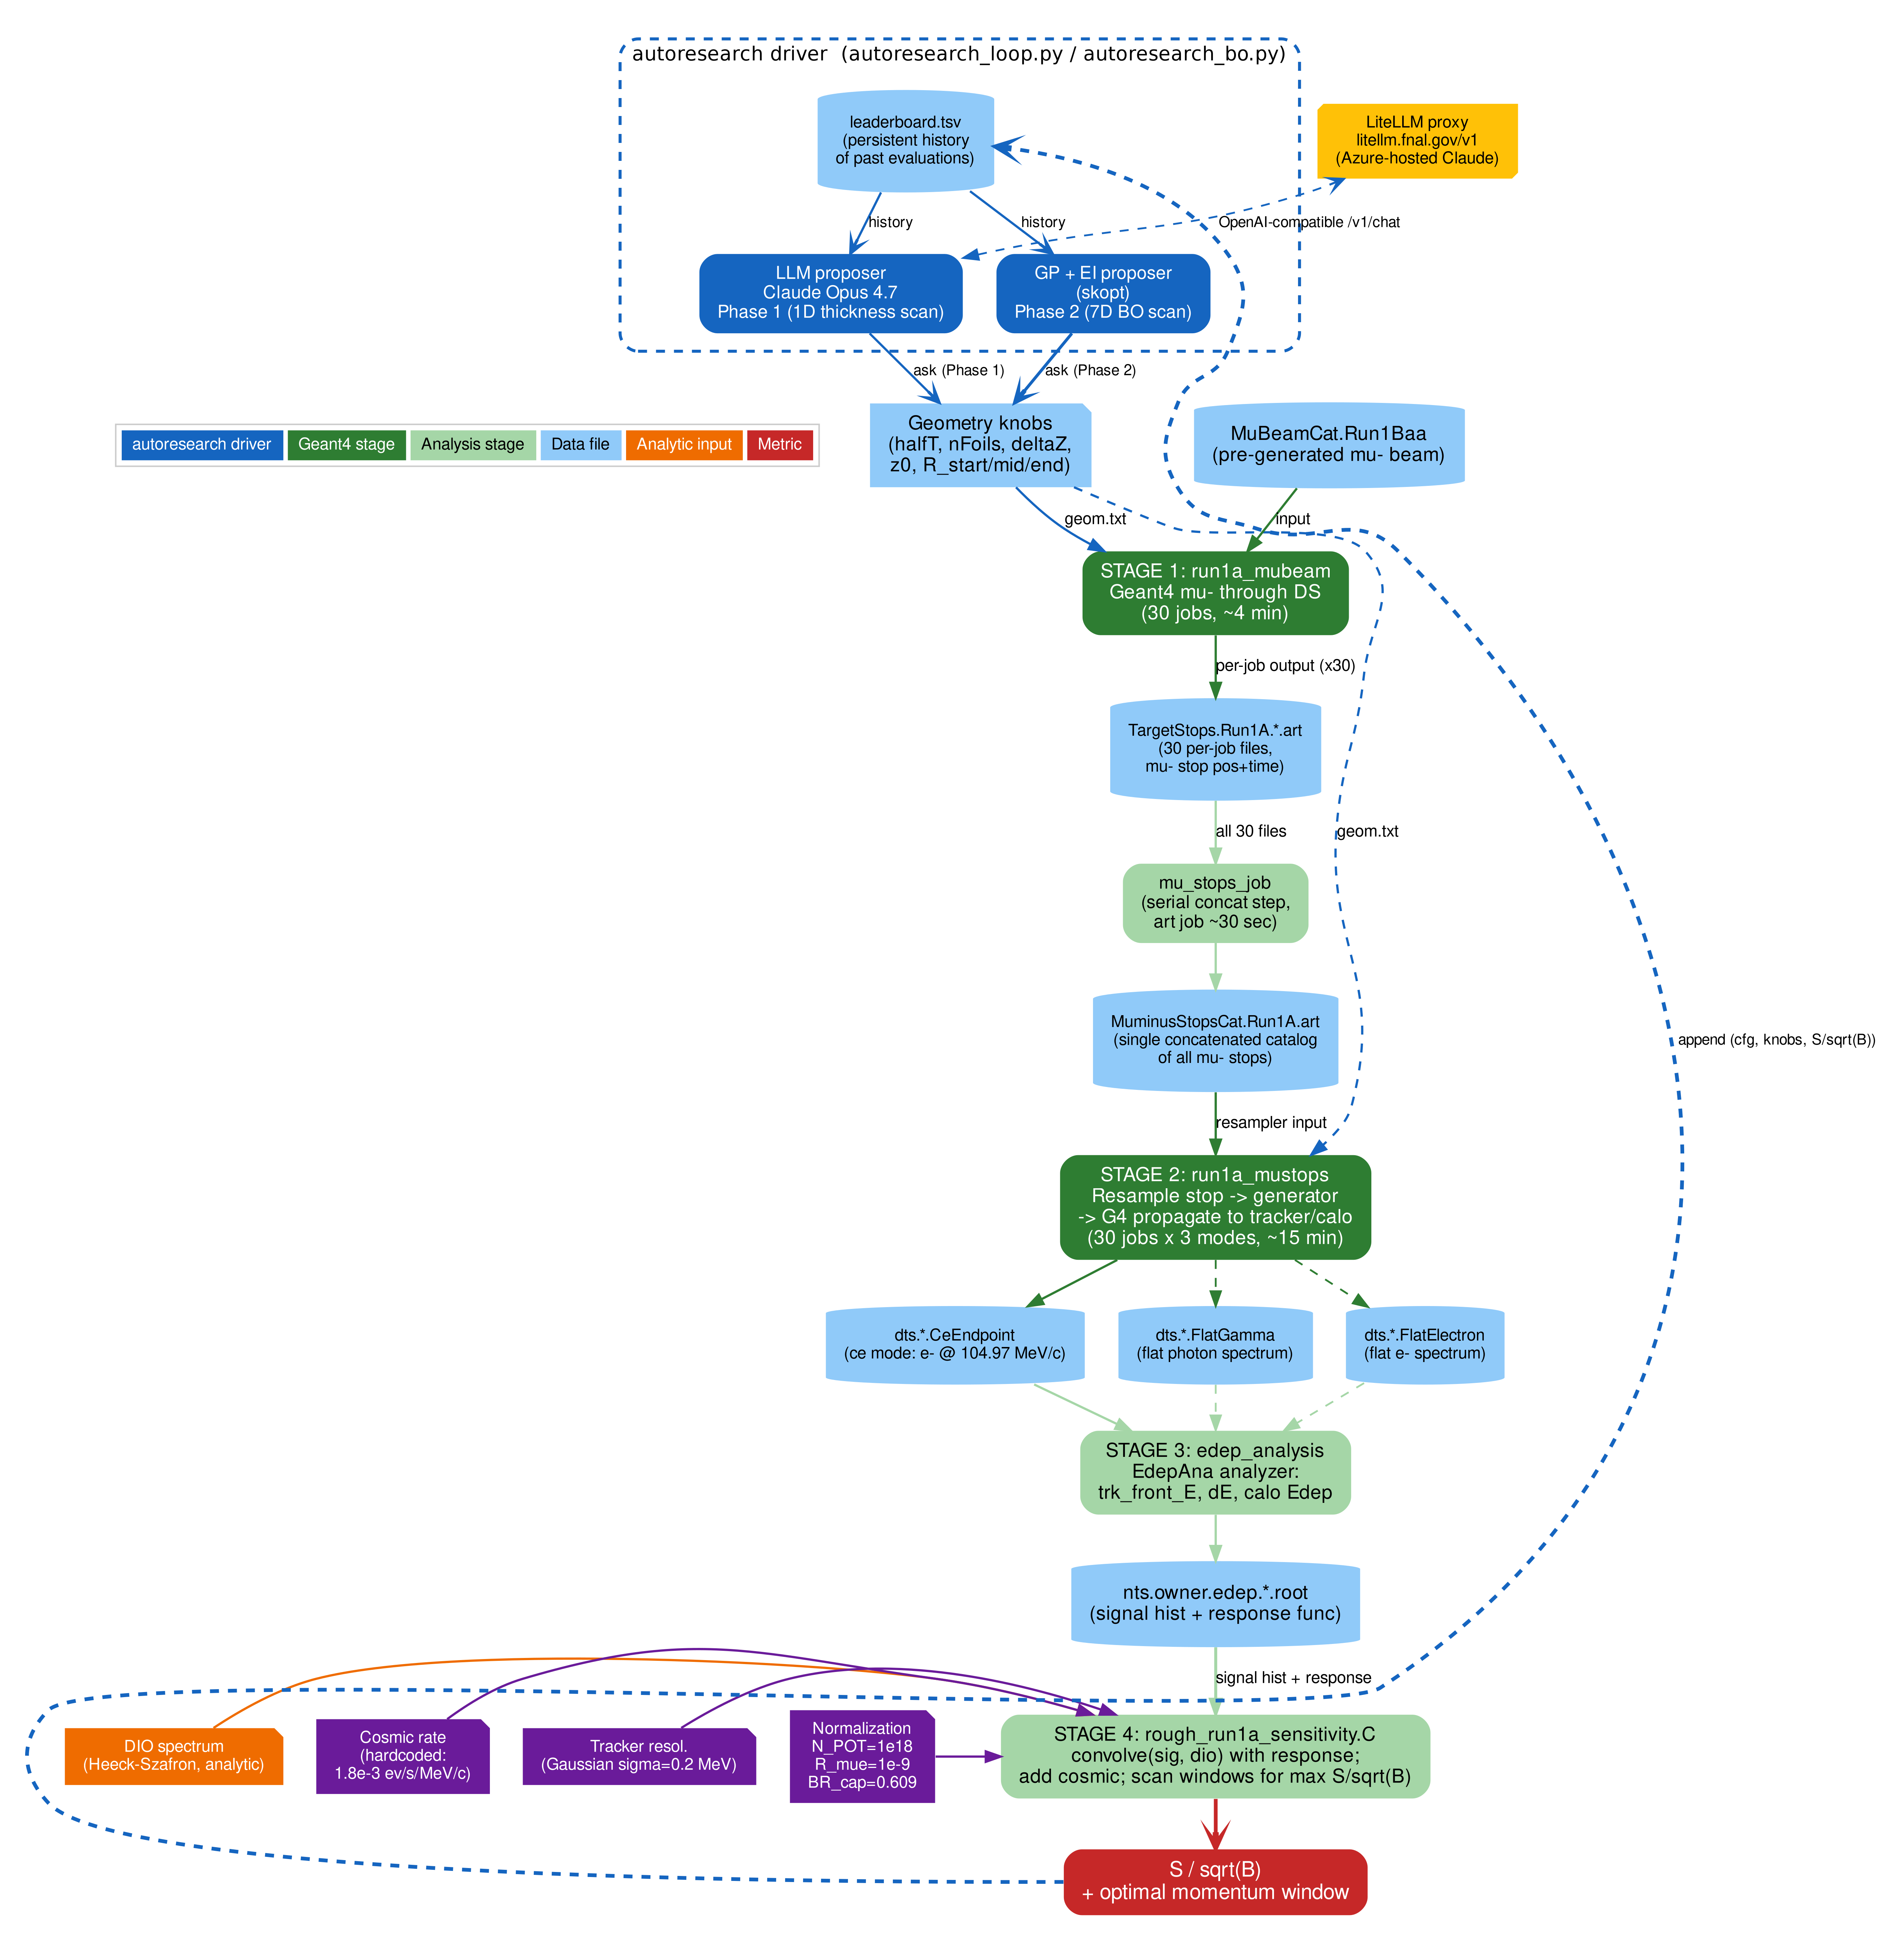
\includegraphics[height=0.75\textheight,keepaspectratio]{pipeline_diagram.png}

\smallskip
{\footnotesize
Top: \textbf{autoresearch driver} (dashed cluster) -- leaderboard + selectable proposer
(LLM via LiteLLM in Phase 1, GP+EI BO in Phase 2).
Middle: Geant4 stages 1--2.
Bottom: analysis stages 3--4.
Loop closes via \texttt{leaderboard.tsv}.
}
\end{frame}

% ----------------------------------------------------------------
\begin{frame}{Key physics points and what BO moves}
\textbf{The CE generator is ``triggered.''} Every $\mu^-$ stop emits an $e^-$ at
endpoint kinematics; we don't wait for real $\mu \to e$ conversion (BR $\sim 10^{-15}$).
The macro scales this artificial population by $R_{\mu e} = 10^{-9}$ and
$N(\mathrm{POT}) = 10^{18}$ to get an absolute event count.

\medskip
\textbf{Stages 1 \& 2 are decoupled} via \texttt{MuminusStopsCat}: mubeam runs once per
geometry; mustops resamples the catalog 3 times (one per generator mode).

\medskip
\textbf{Cosmic and DIO never touch Geant4.}
\begin{itemize}\itemsep=0pt
\item Cosmic: hardcoded flat distribution $\times$ assumed rate
\item DIO: Heeck-Szafron analytic spectrum, convolved with response
\end{itemize}
$\Rightarrow$ all geometry-driven gains move only through
\emph{signal acceptance} $\div$ \emph{window width}.

\medskip
\textbf{What the BO actually moves:}
\smallskip
\begin{center}
geometry knobs $\;\to\;$ ($\mathtt{sig\_eff}$, signal-spectrum shape) $\;\to\; S/\sqrt{B}$
\end{center}

\smallskip
\begin{itemize}\itemsep=0pt
\item \texttt{halfT, nFoils, deltaZ, z0} -- change \emph{how many} $\mu^-$ stop and \emph{where}
\item \texttt{R\_start, R\_mid, R\_end} -- change \emph{which} $\mu^-$ stop (off-axis acceptance)
\item All knobs feed Stages 1+2; Stages 3+4 are deterministic post-processing
\end{itemize}
\end{frame}

% ----------------------------------------------------------------
\begin{frame}{Baselines}
Three runs of the default 37-foil target ($t_{1/2}=0.0528$ mm):

\medskip
\begin{tabular}{lcc}
\toprule
Run & Window (MeV/c) & $S/\sqrt{B}$ \\
\midrule
Mike's \texttt{config\_v00} (Apr 18) & $[104.5, 104.5]$  & 3.35 \\
Our \texttt{config\_v24} (yesterday) & $[103.9, 104.7]$  & 3.34 \\
Our \texttt{config\_v00} (today)     & $[103.9, 104.7]$  & 3.31 \\
\bottomrule
\end{tabular}

\medskip
Cross-validates the pipeline. All three within $\sim$1\% (MC noise).
\end{frame}

% ----------------------------------------------------------------
\begin{frame}{Phase 1: 1D scan over foil half-thickness (LLM-greedy)}
\textbf{Single knob:} \texttt{stoppingTarget.halfThicknesses} $\in [0.025, 0.150]$ mm.
\smallskip

\textbf{Loop} (10 iterations, $\sim$3.5 h total):
\begin{enumerate}
\item Read leaderboard (history)
\item LLM (\texttt{azure/claude-opus-4-7} via \texttt{litellm.fnal.gov/v1}) proposes next $t$
\item Fork config, write geom override, run pipeline ($\sim$20 min)
\item Parse $S/\sqrt{B}$, append to leaderboard
\end{enumerate}

\medskip
LLM behavior: 3-point spread to characterize, then bisect around best.
\end{frame}

% ----------------------------------------------------------------
\begin{frame}{Phase 1 results: 7 successful evaluations}
\centering
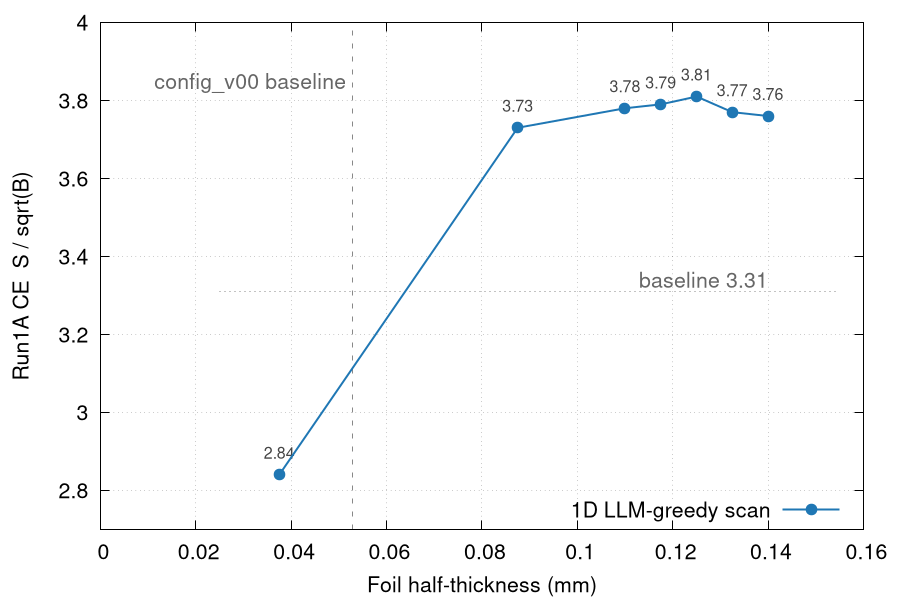
\includegraphics[width=0.70\linewidth]{thickness_scan.png}

\smallskip
\textbf{Best: $t_{1/2}=0.125$ mm, $S/\sqrt{B}=3.81$} \quad ($+15\%$ vs.\ baseline 3.31)

Plateau: $S/\sqrt{B}\!\in\![3.76,3.81]$ for $t_{1/2}\!\in\![0.110, 0.140]$ mm
\end{frame}

% ----------------------------------------------------------------
\begin{frame}{Why thickness has an optimum}
Two competing effects:

\smallskip
\begin{itemize}
\item Thicker foils $\Rightarrow$ more $\mu^-$ stops $\Rightarrow$ \emph{linear} signal gain
\item Thicker foils $\Rightarrow$ more $E$-loss + multiple scattering before
      tracker $\Rightarrow$ broader CE peak $\Rightarrow$ optimal window widens
      $\Rightarrow$ more cosmic bkg
\end{itemize}

\medskip
\begin{tabular}{lccc}
\toprule
$t_{1/2}$ (mm) & Window width (MeV/c) & Signal & Cosmic \\
\midrule
0.0375 & 0.8 & 39 & 190 \\
0.0875 & 1.2 & 61 & 270 \\
\textbf{0.1250} & \textbf{1.8} & \textbf{75} & \textbf{390} \\
0.1400 & 2.0 & 77 & 420 \\
\bottomrule
\end{tabular}

\smallskip
$0.0375\!\to\!0.125$ mm: signal $\times1.9$, cosmic $\times2.0$ \\
$\Rightarrow S/\sqrt{B} \times 1.34$ (matches: $2.84 \to 3.81$)
\end{frame}

% ----------------------------------------------------------------
\begin{frame}{Phase 2: 7D Bayesian Optimization}
\textbf{Knob set:}

\smallskip
\begin{tabular}{lll}
\toprule
Knob & Range & Type \\
\midrule
\texttt{halfT}      & $[0.025, 0.150]$ mm & continuous \\
\texttt{nFoils}     & $[20, 60]$          & integer \\
\texttt{deltaZ}     & $[10, 30]$ mm       & continuous \\
\texttt{z0}         & $[5700, 6200]$ mm   & continuous \\
\texttt{R\_start}   & $[50, 100]$ mm      & cont.\ (foil 0) \\
\texttt{R\_mid}     & $[50, 100]$ mm      & cont.\ (foil $N/2$) \\
\texttt{R\_end}     & $[50, 100]$ mm      & cont.\ (foil $N{-}1$) \\
\bottomrule
\end{tabular}

\medskip
\textbf{Outer-radius profile:} quadratic Lagrange interpolation through 3 control points
$\Rightarrow$ smooth taper / bulge / inverse-taper with only 3 BO knobs.

\smallskip
\textbf{Constraints:} $z_0 + (n_{\mathrm{foils}}-1)\,\Delta z \leq 6500$ mm;
\texttt{stoppingTarget.holeRadius} fixed at 21.5 mm.
\end{frame}

% ----------------------------------------------------------------
\begin{frame}{BO setup}
\begin{itemize}
\item \texttt{scikit-optimize} GP regressor + Expected Improvement acquisition
\item Seeded with the 7 thickness priors $\Rightarrow$ GP starts with data along one axis
\item Budget: \textbf{40 fresh evaluations}, completed in $\sim$15 hours wall-clock
\item Driver: \texttt{autoresearch\_bo.py}, resumable from \texttt{leaderboard\_bo.tsv}
\item Validation phase planned: top-3 candidates re-run at $50\,k$ events/job
\end{itemize}

\medskip
\textbf{Why surrogate at this stage?}
\begin{itemize}
\item 1D: surrogate overkill, LLM-greedy or sweep is fine
\item 5D--7D: vanilla BO converges in $\sim 30$--$40$ trials at this dimensionality
\item Effective dim is low: physics smoothness encoded by the quadratic basis
\end{itemize}
\end{frame}

% ----------------------------------------------------------------
\begin{frame}{Phase 2 results: convergence}
\centering
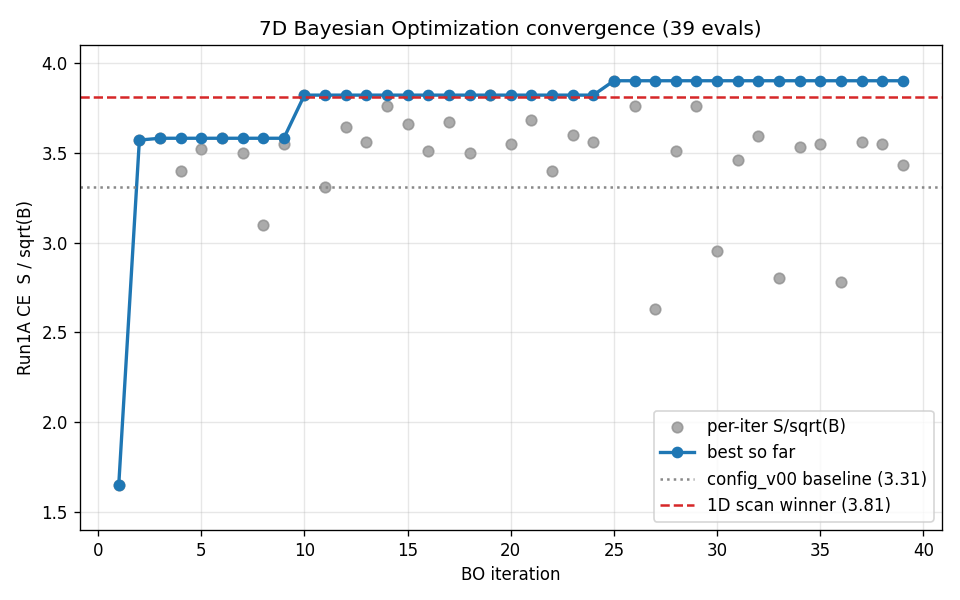
\includegraphics[width=0.72\linewidth]{bo_convergence.png}

\smallskip
\textbf{Best: \texttt{config\_bo025}, $S/\sqrt{B} = 3.90$}\;($+18\%$ vs.\ baseline, $+2.4\%$ vs.\ 1D winner)

\smallskip
{\footnotesize
Iter 1: extreme corner ($1.65$, informative failure).\;
Iter 10: matches 1D winner.\;
Iter 25: finds 3.90.\;
Iters 26--40: plateau.
}
\end{frame}

% ----------------------------------------------------------------
\begin{frame}{Phase 2 results: best configuration}
\textbf{config\_bo025} vs.\ baseline:

\medskip
\begin{tabular}{lcc}
\toprule
Knob & \texttt{config\_v00} (baseline) & \texttt{config\_bo025} \\
\midrule
\texttt{halfT}     & 0.0528 mm & \textbf{0.0842 mm} \\
\texttt{nFoils}    & 37        & \textbf{39} \\
\texttt{deltaZ}    & 22.22 mm  & \textbf{16.71 mm} \\
\texttt{z0}        & 5871 mm   & \textbf{5755 mm} \\
\texttt{R\_start}  & 75 mm     & 84.6 mm \\
\texttt{R\_mid}    & 75 mm     & \textbf{97.8 mm} \\
\texttt{R\_end}    & 75 mm     & 96.3 mm \\
\midrule
\textbf{$S/\sqrt{B}$} & \textbf{3.31} & \textbf{3.90} \quad ($+18\%$) \\
\bottomrule
\end{tabular}

\medskip
Top 3 (within MC noise of each other): \\
\texttt{bo025} (3.90), \texttt{bo009} (3.82), \texttt{bo019} (3.82) -- statistically tied.
\end{frame}

% ----------------------------------------------------------------
\begin{frame}{Phase 2 results: per-knob projections}
\centering
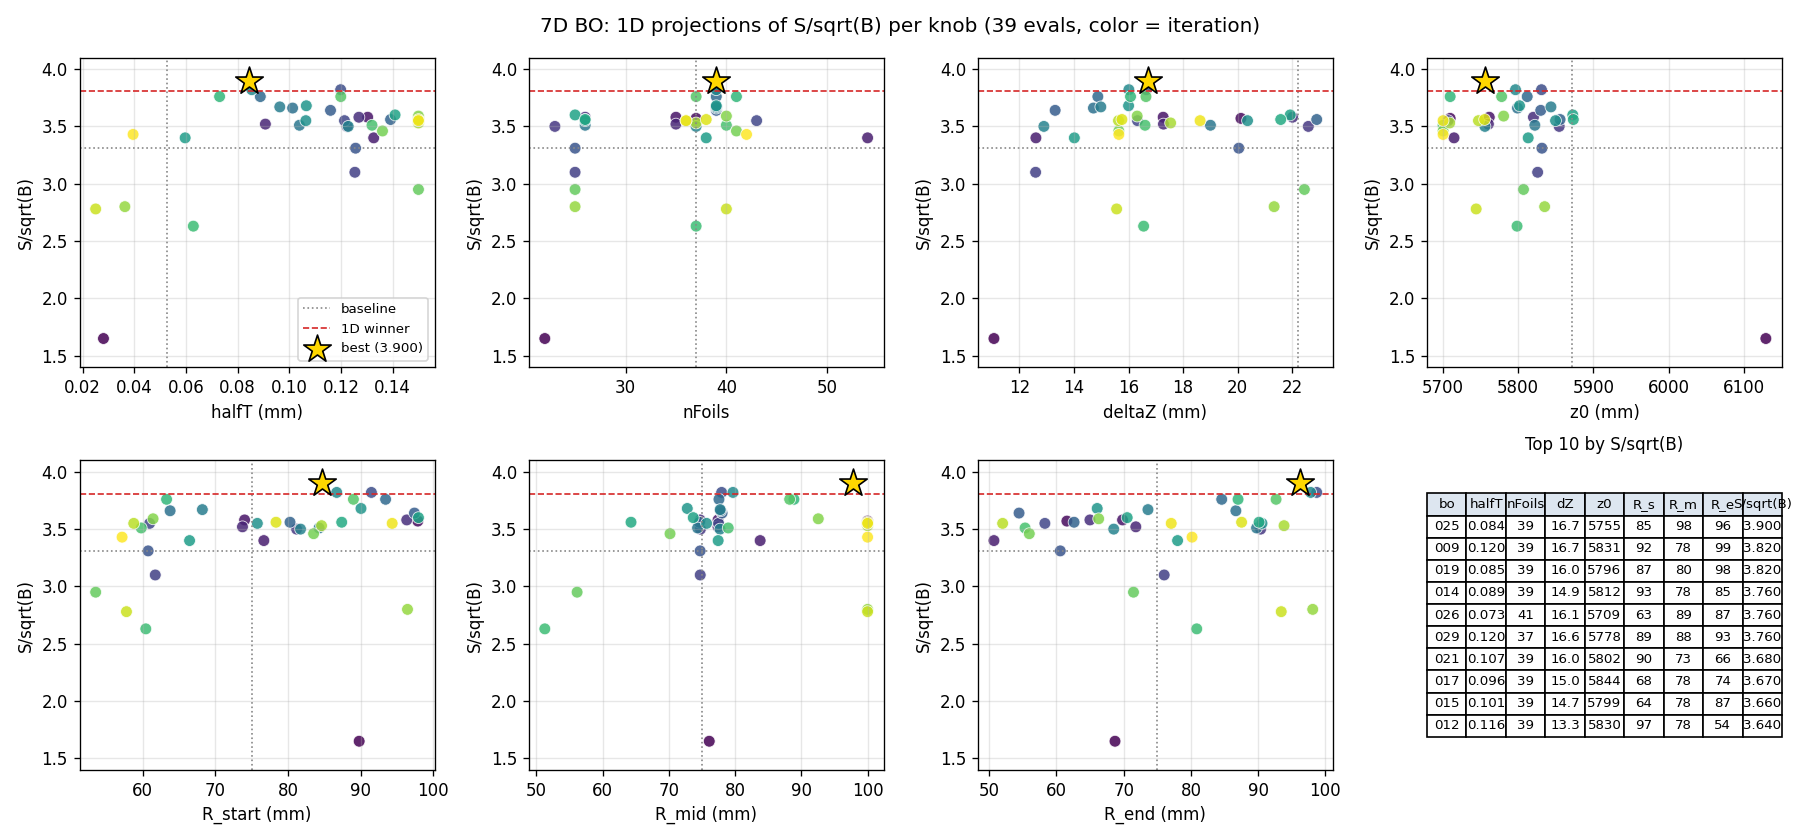
\includegraphics[width=\linewidth]{bo_projections.png}

\smallskip
{\small
Color: BO iteration. Star: best ($S/\sqrt{B}=3.90$). Dotted vertical: baseline.
Dashed horizontal: 1D-scan winner (3.81).
}
\end{frame}

% ----------------------------------------------------------------
\begin{frame}{Which knobs actually mattered?}
After-the-fact regression on 39 evaluations (excluding the 1.65 corner outlier):

\medskip
\begin{tabular}{lccc}
\toprule
Knob & $R^2$ (linear, alone) & top-10 range used & verdict \\
\midrule
\texttt{R\_start}  & \textbf{0.155} & 68\% of [50,100] & weak constraint \\
\texttt{halfT}     & 0.115 & 38\% of [0.025,0.150] & moderate \\
\texttt{nFoils}    & 0.059 & \textbf{10\% of [20,60]} & strongly converged (37--41) \\
\texttt{R\_mid}    & 0.032 & 50\% & weak \\
\texttt{deltaZ}    & 0.012 & \textbf{17\% of [10,30]} & strongly converged (13--17) \\
\texttt{z0}        & 0.002 & 27\% & moderate \\
\texttt{R\_end}    & \textbf{0.000} & 89\% & \textbf{essentially flat} \\
\bottomrule
\end{tabular}

\medskip
\textbf{Linear fit, all 7 knobs together:} $R^2 = 0.42$.
The other 58\% is nonlinear / coupling / MC noise.

\smallskip
\textbf{Key takeaway:} 2 of 7 knobs (\texttt{nFoils}, \texttt{deltaZ}) are tightly
converged; the radius profile (\texttt{R\_*}) contributes weakly.
\texttt{R\_end} can be dropped from any future scan -- it is genuinely
unconstrained, not under-sampled.
\end{frame}

% ----------------------------------------------------------------
\begin{frame}{Why more 7D iterations won't help}
Three independent reasons combined:

\medskip
\begin{enumerate}
\item \textbf{Physics ceiling.} $S/\sqrt{B} = $ signal $/ \sqrt{\mathrm{cosmic}}$, with cosmic
hard-coded. Geometry can only improve signal acceptance / window width;
the 1D scan already approached the ceiling.

\item \textbf{Noise floor.} Per-eval noise $\sim 2\%$ on $S/\sqrt{B}$.
Top-3 spread (3.90, 3.82, 3.82) is at noise. Iter 41 returning 3.95
would be statistically indistinguishable from 3.90.

\item \textbf{BO has converged.} 15 iterations after iter 25 produced no
improvement. Late iterations sampled known corners (e.g.\ \texttt{R\_mid=100, halfT=0.15})
returning $\sim 3.55$, well below 3.90.
\end{enumerate}

\medskip
\textbf{Slice test} (configs with \texttt{nFoils}$\in$[37,41] and \texttt{deltaZ}$\in$[14,18],
$N=17$): $S/\sqrt{B}$ mean = 3.55, max = 3.90.
The remaining 5 knobs vary widely within this slice but the maximum
is still 3.90.

\medskip
$\Rightarrow$ \emph{This 7D box has been effectively explored.}
Real gains require changing the problem -- new dimensions or different
analysis.
\end{frame}

% ----------------------------------------------------------------
\begin{frame}{Caveats}
\begin{itemize}
\item \textbf{Cosmic background is hard-coded} in the macro. All gains move
      through (signal acceptance) $\div$ (window width) -- not from cosmic
      modeling improvements.
\item \textbf{MC noise} per evaluation $\sim 1\%$--$2\%$ (30 jobs $\times$ 10\,k events).
      Top points within $\sim 1.5\%$ are statistically tied.
\item \textbf{TSdA = polyethylene neutron absorber} in \texttt{config\_v00}, not the
      Run~1B Al-endplate variant. Adding the endplate knobs would be a
      separate scan ($+$5 dims).
\item \textbf{Run 1B physics not in this study} -- field-off Run~1B
      stages take $\sim$44 min/eval and would change the iteration economics.
\end{itemize}
\end{frame}

% ----------------------------------------------------------------
\begin{frame}{Available knobs beyond the 7D scan}
The Mu2e geometry code (\texttt{StoppingTargetMaker.cc}) supports per-foil specifications
\emph{straight from the geom .txt file} -- no Offline source changes:

\medskip
{\footnotesize
\begin{tabular}{lll}
\toprule
Parameter & Vector type & Currently in BO? \\
\midrule
\texttt{radii} & per-foil outer R & yes (3 knobs, quadratic) \\
\texttt{halfThicknesses} & per-foil thickness & 1 scalar; could go quadratic (3) \\
\texttt{zVars} & per-foil z offset & not used; non-uniform spacing (3) \\
\texttt{xCos} & per-foil tilt (about y) & not used (1 uniform or 3 quad.) \\
\texttt{yCos} & per-foil tilt (about x) & redundant ($\varphi$-symmetric) \\
\texttt{xVars}, \texttt{yVars} & per-foil x,y offset & transverse misalignment \\
\texttt{foilTarget\_support*} & support wires & material / count near foils \\
\bottomrule
\end{tabular}
}

\medskip
Pattern: 3 control points $\to$ quadratic Lagrange $\to$ smooth per-foil profile.
Same 3-knob cost as \texttt{R\_start}, \texttt{R\_mid}, \texttt{R\_end}.
\end{frame}

% ----------------------------------------------------------------
\begin{frame}{Full smooth-target parametrization (theoretical)}
If we promote every per-foil quantity to a quadratic profile:

\medskip
\begin{tabular}{lc}
\toprule
Knob group & BO knobs \\
\midrule
Foil thickness profile (3 control points) & 3 \\
Foil outer radius profile (3 control points) & 3 \\
Foil spacing profile (3 control points) & 3 \\
Foil tilt profile (3 control points, x only) & 3 \\
\texttt{nFoils} & 1 \\
\texttt{z0} (target center) & 1 \\
\midrule
\textbf{Total} & \textbf{14D} \\
\bottomrule
\end{tabular}

\medskip
\textbf{Why y-tilt is excluded:} Mu2e is approximately $\varphi$-symmetric (beam,
solenoid field, tracker, calorimeter all centered on z). x- and y-tilt produce
identical $S/\sqrt{B}$ up to a 90$^{\circ}$ rotation; adding yCos as a BO knob just
explores a redundant circle in (xCos, yCos) space.

\medskip
\textbf{14D budget:} vanilla GP-EI BO needs $\sim$80--120 trials. At 20 min/eval
that's $\sim$30 hours.
Practical: run cheap 1D probes at the current 7D winner to triage which extra knobs deserve to graduate to BO dimensions.
\end{frame}

% ----------------------------------------------------------------
\begin{frame}{Cheap 1D probes (recommended path)}
After the 7D scan converges, run 1D scans at the current best to decide which
knobs are worth promoting:

\medskip
\begin{tabular}{lll}
\toprule
Probe & Cost & Decision rule \\
\midrule
Per-foil thickness (uniform $\to$ tapered) & 5 evals, 1.5 h & promote if $>$2\% on $S/\sqrt{B}$ \\
Per-foil spacing (uniform $\to$ tapered) & 5 evals, 1.5 h & promote if $>$2\% \\
Foil tilt (uniform, $\theta\!\in\![0, 30^\circ]$) & 5 evals, 1.5 h & promote if $>$2\% \\
Support-wire radius & 5 evals, 1.5 h & rarely matters; quick sanity \\
\bottomrule
\end{tabular}

\medskip
$\approx$30 evals $\times$ 20 min = 10 hours total to triage all four. Each
``promoted'' knob group then becomes 3 BO dimensions in a follow-up scan.

\medskip
\textbf{Rationale:} avoid expanding to 11D or 14D BO without evidence that
the extra dims actually move the metric. Cheap to verify, expensive to ignore.
\end{frame}

% ----------------------------------------------------------------
\begin{frame}{Beyond the stopping target}
Knobs we deliberately did \emph{not} include in the autoresearch scan, but worth
noting:

\medskip
\begin{itemize}
\item \textbf{TSdA Run~1B endplate} -- 5 knobs (material, r4, rin, halfLength, z0).
      Currently polyethylene neutron absorber; switching to Al-as-stopping-target is
      a Run~1B physics concept.
\item \textbf{Proton Absorber} (PA / IPA) -- z, inner radius, thickness.
      Sits between target and tracker; affects CE energy loss and resolution.
\item \textbf{Tracker placement} -- \texttt{ds2.halfLength}, \texttt{tracker.inDS2Vacuum}.
\item \textbf{DS field scale factor} -- changes momentum reconstruction.
\item \textbf{Stopping-target material} -- non-Al would change capture branching;
      breaks the analysis assumptions but worth investigating for material studies.
\end{itemize}

\medskip
And on the analysis side:
\begin{itemize}
\item \textbf{Cosmic background model} (currently hard-coded $\sim 1.8\times 10^{-3}$/s/MeV/c).
      Replacing with sim-derived spectrum is the single biggest unknown for absolute $S/\sqrt{B}$.
\item \textbf{Tracker resolution} (currently Gaussian $\sigma\!=\!0.2$ MeV).
\end{itemize}
\end{frame}

% ----------------------------------------------------------------
\begin{frame}{Next steps}
\textbf{Done:}
\begin{itemize}
\item 1D LLM-greedy thickness scan (10 evals, +15\% over baseline)
\item 7D BO over thickness + foil-count + spacing + z + radius profile (40 evals, $+18\%$)
\end{itemize}

\medskip
\textbf{Recommended immediate:}
\begin{enumerate}
\item \textbf{Validate top 3} (\texttt{bo025, bo009, bo019}) at $5\times$ stats (50\,k events/job).
  $\sim$3.75 h. Tells us whether 3.90 is real or a 2\% upfluctuation.
\item \textbf{Promote winner} into a hand-vetted \texttt{config\_v40} once validated.
\end{enumerate}

\medskip
\textbf{Optional follow-ups (to extract gains beyond the cosmic ceiling):}
\begin{itemize}
\item \textbf{Drop \texttt{R\_end}}, add per-foil \emph{thickness} profile (3 knobs) and
      per-foil \emph{spacing} profile (3 knobs) $\to$ 11D BO with new physics axes
\item \textbf{Add TSdA Al-endplate knobs} $\to$ Run~1B endplate variant
\item \textbf{Replace hard-coded cosmic} with sim-derived spectrum (analysis-side change)
\item \textbf{Extend to Run~1B \texttt{final}-stage CE sensitivity}
      (full pipeline, $\sim$44 min/eval, field-off regime)
\end{itemize}
\end{frame}

\end{document}
